\section{Error analysis and discussion}
\label{sec:error}

\subsection{Mask quality and recognition}

Across thirteen experiments -- every capacity, resolution and architecture tried --
the quality of matched masks (SQ) moved inside $0.66$--$0.68$ and no further,
against a matched-pair agreement between human annotators of $0.59$; Dice too
passed pairwise annotator agreement ($0.62$) at the second experiment and barely
moved afterwards. This does not close the boundary question: the consensus oracle
of Section~\ref{sec:data} sits at $0.81$, so the headroom is real. What it says is
that \textbf{none of the variables we moved touches it}: capacity, resolution and
loss change \emph{which} filaments we find, not how well we draw them. Every
remaining point of PQ goes through recognition: finding more of the filaments
annotators marked, predicting fewer they did not.

\subsection{False negatives and false positives}

Table~\ref{tab:errors} sorts every error of the delivered model by cause. Instance
recall falls sharply with size, from $0.31$ below 500 pixels to $0.73$ above 5000:
what we miss are small, faint filaments. Split and merge errors together are only
$5.4\%$ of all errors, which is why we never built any split/merge machinery -- the
prize was too small to be worth the code.

\begin{table}[ht]
    \centering
    \caption{Every error of the delivered model on validation, by cause.}
    \label{tab:errors}
    \small\begin{tabular}{llrl}
        \toprule
        & Cause & Count & What it means \\
        \midrule
        \multirow{3}{*}{FN (442)}
          & pure miss   & 193 & not one predicted pixel on the instance \\
          & near miss   & 215 & a blob is there, but IoU stays $\le 0.5$ \\
          & split       & 34  & the filament is found, but in pieces \\
        \midrule
        \multirow{3}{*}{FP (523)}
          & hallucination & 209 & no annotated pixel touched \\
          & unmatched     & 296 & on an annotated filament, but below IoU $0.5$ \\
          & merge         & 18  & one prediction covering two annotations \\
        \bottomrule
    \end{tabular}
\end{table}

Two caveats were checked. First, the organisers confirmed the annotations are
\emph{incomplete}, so part of the hallucinations are plausibly real filaments that
one or more annotators missed -- measured, blobs peaking above $0.85$ probability
are marked by only $63\%$ of annotators, and several probability-map blobs in
Figure~\ref{fig:predictions} sit on structures no annotator drew. Second, the
matching structure the challenge's judging committee inspects is nearly one-to-one
(Figure~\ref{fig:distributions}): of 1144 annotated instances 951 are touched by at
least one prediction and only 81 by more than one.

\begin{figure}[ht]
    \centering
    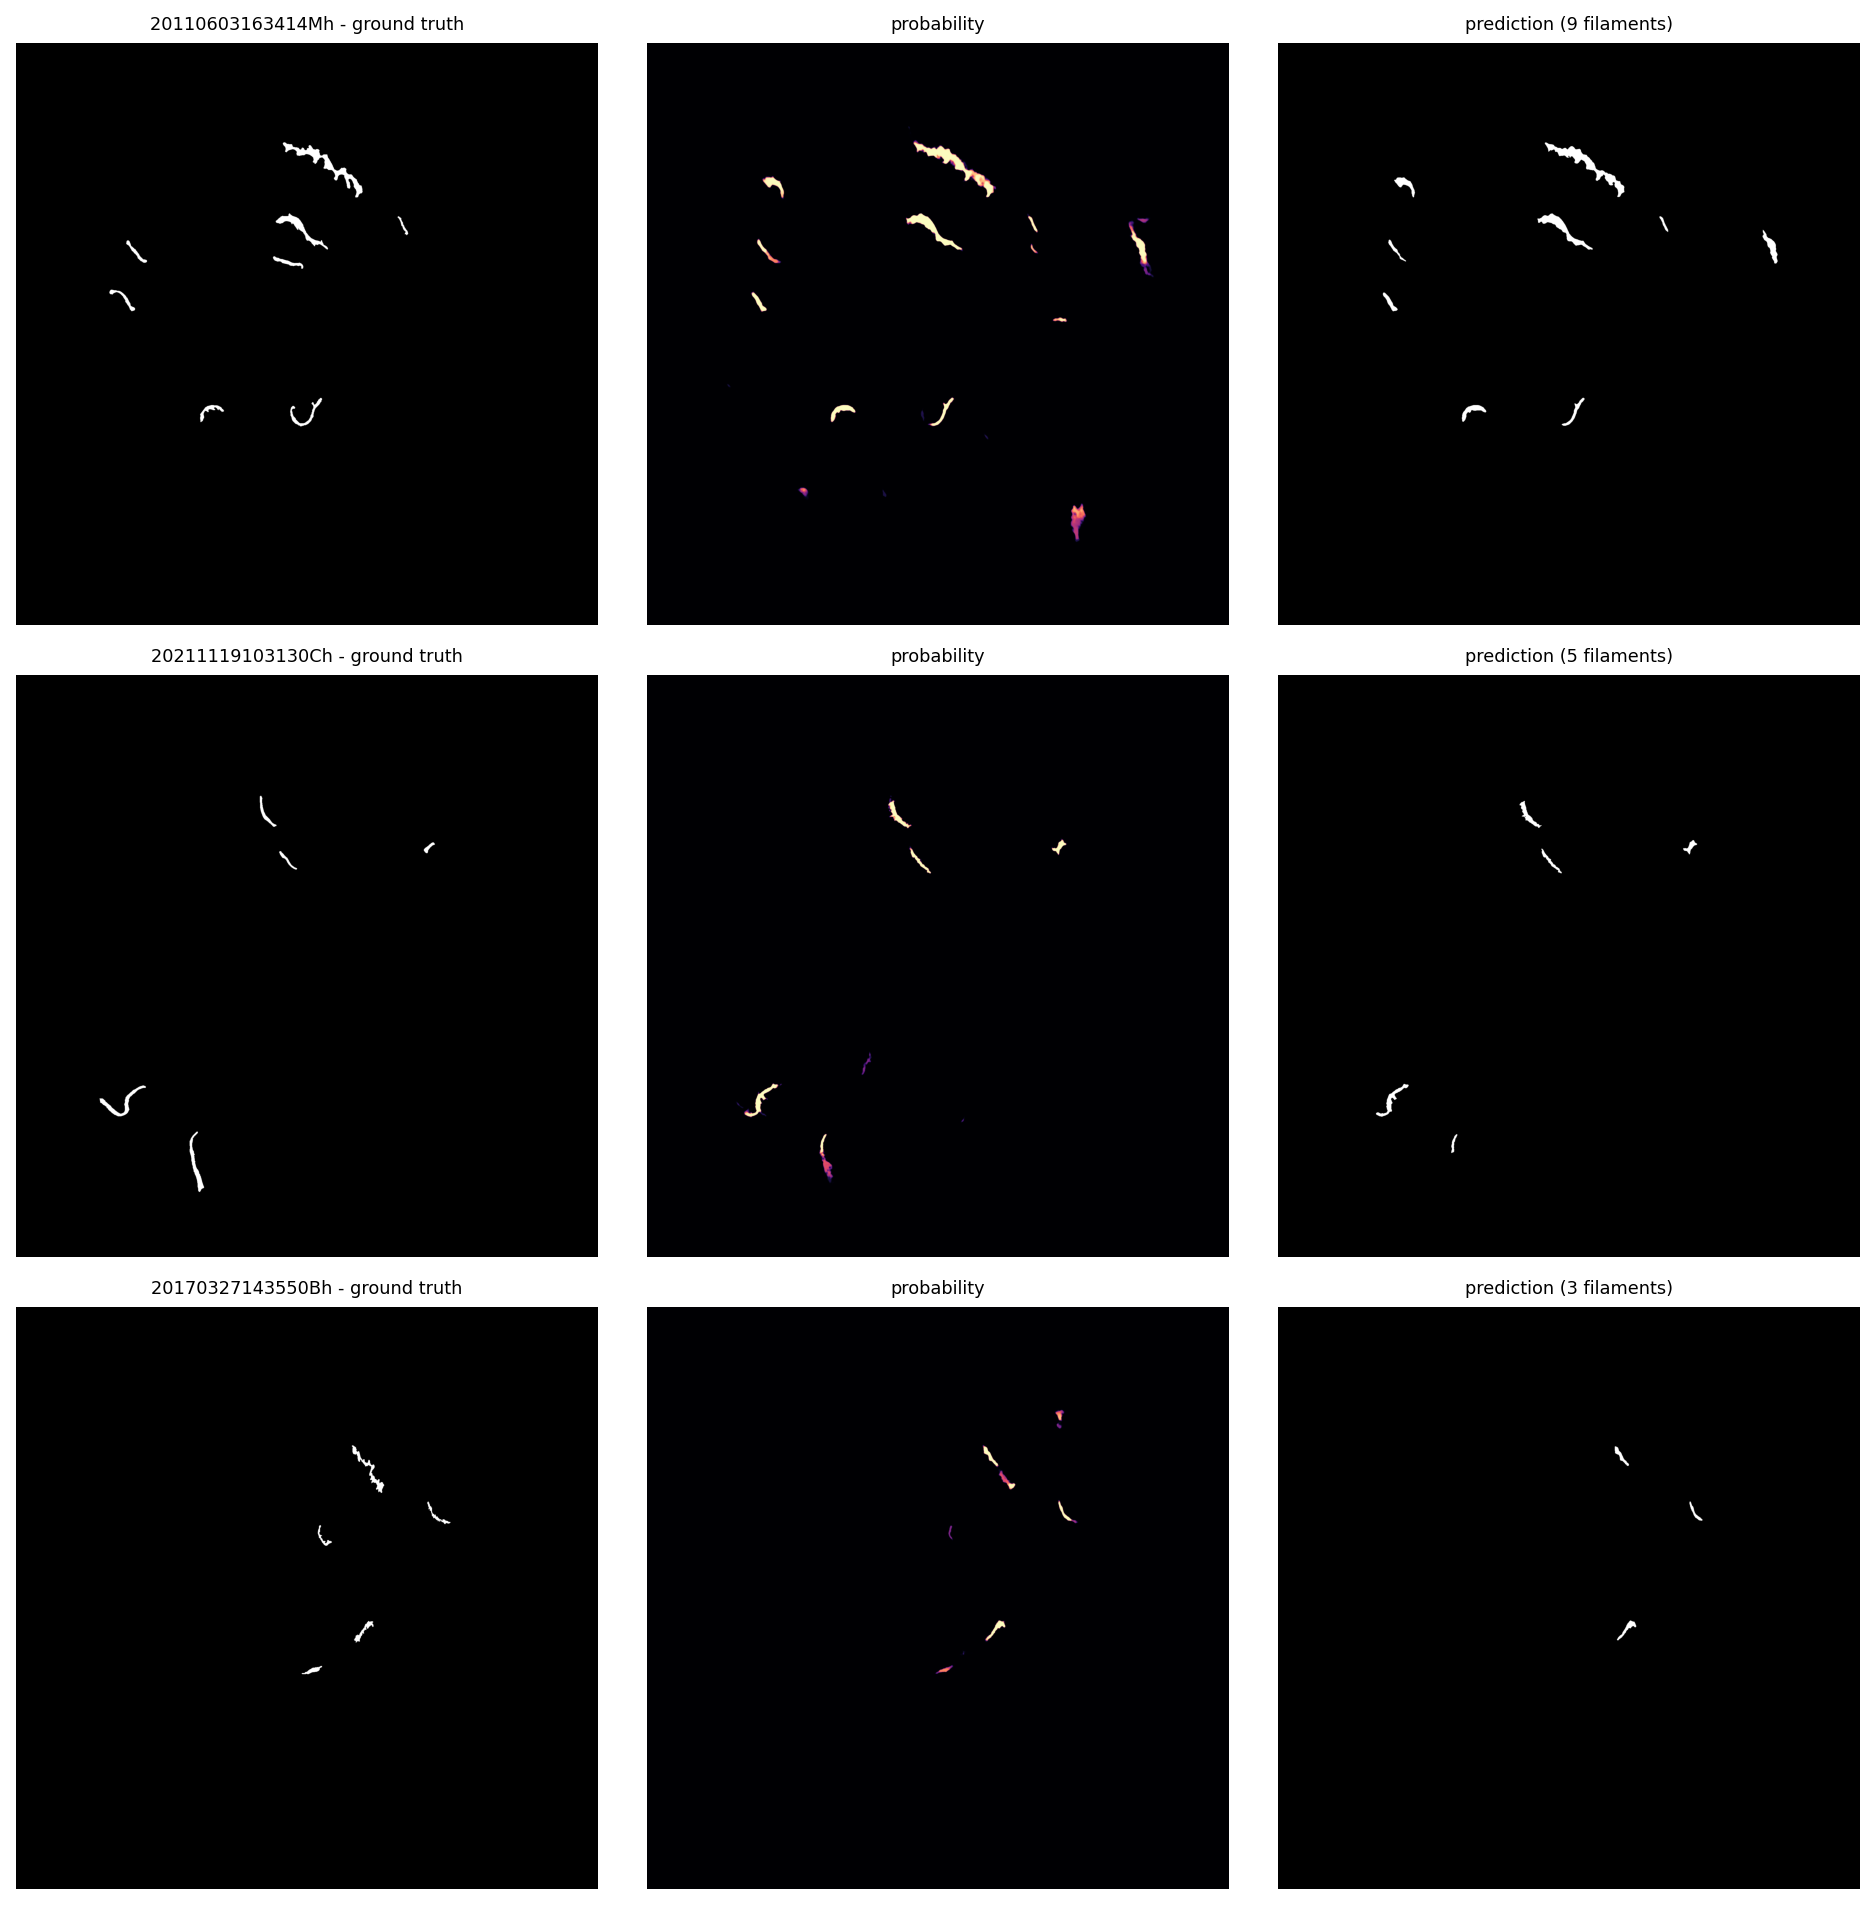
\includegraphics[width=0.86\linewidth]{../experiments/13/plots/validation_predictions.png}
    \caption{The delivered model on three validation observations: annotator ground
    truth (left), predicted probability map (centre), final instances at the
    delivered operating point (right). Several blobs in the probability maps sit on
    structures no annotator drew.}
    \label{fig:predictions}
\end{figure}


\begin{figure}[ht]
    \centering
    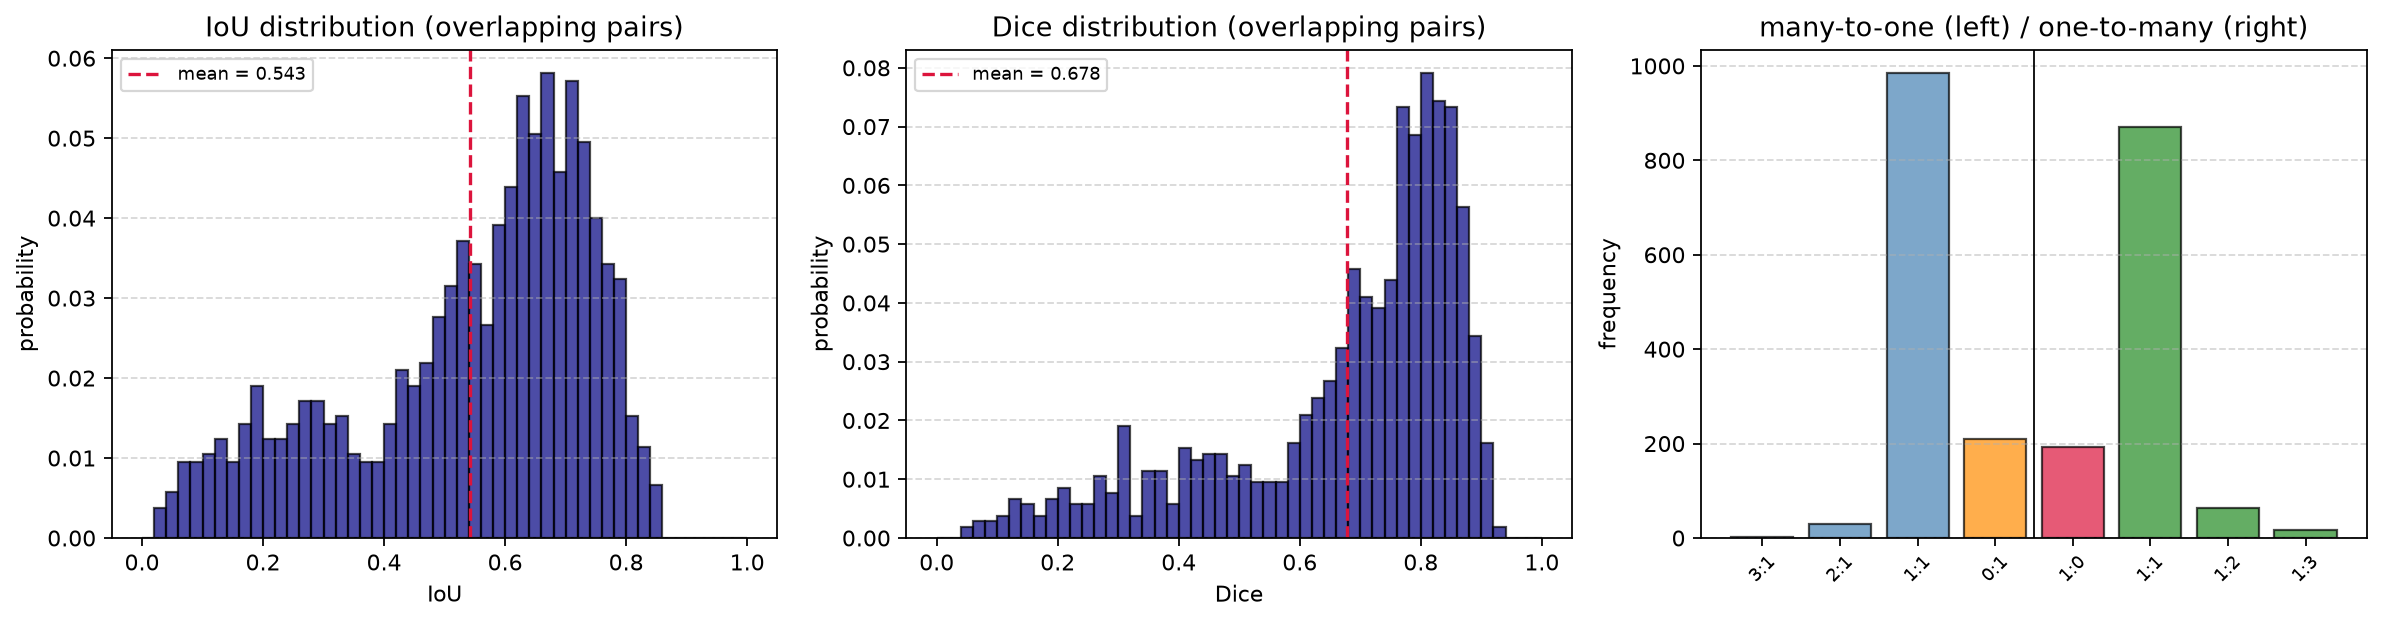
\includegraphics[width=0.98\linewidth]{../experiments/13/plots/official_distributions.png}
    \caption{The distributions reported by the organisers' self-evaluation
    notebook, for the delivered model on validation: IoU and Dice over every
    overlapping ground-truth/prediction pair, and the many-to-one / one-to-many
    relations (a hit is any overlap; the metric's IoU $> 0.5$ gate is stricter).}
    \label{fig:distributions}
\end{figure}

\subsection{Maximising PQ for the Kaggle leaderboard}
\label{sec:kaggle}

With the memory bonus deliberately set aside, the recognition problem was pushed as
far as it would go, and the public leaderboard tracked validation PQ minus a stable
$0.072 \pm 0.007$ across eight submissions -- validation was a reliable compass
throughout. Native $2048$ full-frame models (ResNet18 and ResNet34 encoders) match
the champion; averaging the probability maps of the two \emph{near-equal,
oppositely-biased, different-scale} models beats both under cross-selection
(PQ 0.4354), where every other ensembling attempt had failed; and appending the
confident detections of a YOLOv8x detector wherever the ensemble left pixels free
adds the filaments the pixel-wise models miss entirely (PQ \textbf{0.4414},
cross-validated, public leaderboard \textbf{0.37}). These configurations use up to
9--39~GB in training and are documented here as a study on the Kaggle challenge's
metric; the model we deliver for the project work remains the budget-compliant
Dice optimum of Section~\ref{sec:operating}.
